% ----------------------------------------------------
% DAB Standard
% ----------------------------------------------------
\documentclass[class=report,11pt,crop=false]{standalone}
% Page geometry
\usepackage[a4paper,margin=25mm,top=25mm,bottom=25mm]{geometry}

% Font choice
\usepackage{lmodern}

% Use IEEE bibliography style
\bibliographystyle{IEEEtran}

% Line spacing
\usepackage{setspace}
\setstretch{1.20}

% Ensure UTF8 encoding
\usepackage[utf8]{inputenc}

% Language standard (not too important)
\usepackage[english]{babel}

% Skip a line in between paragraphs
\usepackage{parskip}

% For the creation of dummy text
\usepackage{blindtext}

% Math
\usepackage{amsmath}

% Header & Footer stuff
\usepackage{fancyhdr}
\pagestyle{fancy}
\fancyhead{}
\fancyhead[R]{\nouppercase{\rightmark}}
\fancyfoot{}
\fancyfoot[C]{\thepage}
\renewcommand{\headrulewidth}{0.0pt}
\renewcommand{\footrulewidth}{0.0pt}
\setlength{\headheight}{13.6pt}

% Page geometry
\usepackage[a4paper,top=25mm,bottom=25mm]{geometry}

% Epigraphs
\usepackage{epigraph}
\setlength\epigraphrule{0pt}

% Hyperlinks & References
\usepackage{hyperref}
\hypersetup{
    colorlinks=true,
    linkcolor=blue,
    filecolor=blue,      
    urlcolor=blue,
    citecolor=blue,
}
\urlstyle{same}

% Automatically correct front-side quotes
\usepackage[autostyle=false, style=american]{csquotes}
\MakeOuterQuote{"}

% Graphics
\usepackage{graphicx}
\graphicspath{{Images/}{../Images/}}

% Colour
\usepackage{color}
\usepackage[usenames,dvipsnames]{xcolor}

% SI units
\usepackage{siunitx}

% Microtype goodness
\usepackage{microtype}

% Listings
\usepackage{listings}
\definecolor{backgroundColour}{RGB}{250,250,250}
\definecolor{commentColour}{RGB}{73, 175, 102}
\definecolor{identifierColour}{RGB}{196, 19, 66}
\definecolor{stringColour}{RGB}{252, 156, 30}
\definecolor{keywordColour}{RGB}{50, 38, 224}
\definecolor{lineNumbersColour}{RGB}{127,127,127}
\lstset{ 
  language=Matlab,
  captionpos=b,
  backgroundcolor=\color{backgroundColour},
  basicstyle=\footnotesize,        % the size of the fonts that are used for the code
  breakatwhitespace=false,         % sets if automatic breaks should only happen at whitespace
  breaklines=true,                 % sets automatic line breaking
  postbreak=\mbox{\textcolor{red}{$\hookrightarrow$}\space},
  commentstyle=\color{commentColour},    % comment style
  identifierstyle=\color{identifierColour},
  stringstyle=\color{stringColour},
   keywordstyle=\color{keywordColour},       % keyword style
  %escapeinside={\%*}{*)},          % if you want to add LaTeX within your code
  extendedchars=true,              % lets you use non-ASCII characters; for 8-bits encodings only, does not work with UTF-8
  frame=single,	                   % adds a frame around the code
  keepspaces=true,                 % keeps spaces in text, useful for keeping indentation of code (possibly needs columns=flexible)
  morekeywords={*,...},            % if you want to add more keywords to the set
  numbers=left,                    % where to put the line-numbers; possible values are (none, left, right)
  numbersep=5pt,                   % how far the line-numbers are from the code
  numberstyle=\tiny\color{lineNumbersColour}, % the style that is used for the line-numbers
  rulecolor=\color{black},         % if not set, the frame-color may be changed on line-breaks within not-black text (e.g. comments (green here))
  showspaces=false,                % show spaces everywhere adding particular underscores; it overrides 'showstringspaces'
  showstringspaces=false,          % underline spaces within strings only
  showtabs=false,                  % show tabs within strings adding particular underscores
  stepnumber=1,                    % the step between two line-numbers. If it's 1, each line will be numbered
  tabsize=2,	                   % sets default tabsize to 2 spaces
  %title=\lstname                   % show the filename of files included with \lstinputlisting; also try caption instead of title
}

% Caption stuff
\usepackage{caption}
\usepackage{subcaption}

\makenoidxglossaries

\newacronym{radar}{RADAR}{Radio Detection and Ranging}
\newacronym{dab}{DAB}{Digital Audio Broadcasting}
\newacronym{fm}{FM}{Frequency Modulation}
\newacronym{am}{AM}{Amplitude Modulation}
\newacronym{fdm}{FDM}{Frequency Division Multiplexing}
\newacronym{ofdm}{OFDM}{Orthogonal Frequency Division Multiplexing}
\newacronym{cofdm}{COFDM}{Coded Orthogonal Frequency Division Multiplexing}
\newacronym{dvbt2}{DVB–T2}{Digital Video Broadcasting — Second Generation Terrestrial}
\newacronym{em}{EM}{electromagnetic}
\newacronym{icasa}{ICASA}{Independent Communications Authority of South Africa}
\newacronym{ioo}{IOO}{Illuminators of Opportunity}
\newacronym{pr}{PR}{Passive Radar}
\newacronym{qpsk}{QPSK}{Differential Quadrature Phase-Shift Keying}
\newacronym{dqpsk}{DQPSK}{Differential Quadrature Phase-Shift Keying}
\newacronym{etsi}{ETSI}{European Telecommunications Standards Institute}
\newacronym{psk}{PSK}{Phase Shift Keying}
\newacronym{ask}{ASK}{Amplitude-Shift Keying}
\newacronym{fsk}{FSK}{Frequency-Shift Keying}
\newacronym{iq}{IQ}{In-phase and Quadrature}
\newacronym{prs}{PRS}{Phase Reference Symbol}
\newacronym{dft}{DFT}{Discrete Fourier Transform}
\newacronym{fft}{FFT}{Fast Fourier Transform}
\begin{document}
\ifstandalone
\tableofcontents
\fi
% ----------------------------------------------------
\chapter{Digital Audio Broadcasting: Standard}
\epigraph{Where the waters do agree, it is quite wonderful the relief they give.}%
{\emph{---Jane Austen, Emma}}
% ----------------------------------------------------

\section{Overview}
This chapter aims to outline the key components of the \gls{dab} standard, as prescribed by the \gls{etsi} in~\cite{dabstandard}. This begins with a discussion on \gls{cofdm} and \gls{dqpsk}, each of which is fundamental to \gls{dab}. Thereafter, the structure of a \gls{dab} frame will be mentioned, with special highlights made to the null and phase-reference symbols. Note, however, that since this report focuses on \gls{dab} signals within the context of \gls{pr}, it is unnecessary for a complete description of the \gls{dab} format. In fact, massive simplifications can be made. The \gls{dab}-based \gls{pr} chain need not dive into the specifics of the source audio coding, and so on.

\section{Coded Orthogonal Frequency Division Multiplexing}
In 1966, Robert W. Chang published an incredibly important paper~\cite{Chang1966}, outlining the idea of \gls{ofdm}.

\subsection{Motivation}
Suppose one wanted to transmit a set of symbols, \(\mathcal{D}\), using some arbitrary modulation scheme. There are, in essence, two approaches to do this. The first, which is markedly simpler, is a serial approach: simply to modulate a carrier wave with successive elements of \(\mathcal{D}\). Alternatively, one could take a parallel approach. That is, to split \(\mathcal{D}\) into \(n\) subsets, and then use these subsets to modulate \(n\) independent carriers respectively. Figure~\ref{fig:carrier-illustration} illustrates these situations with two simplified spectrograms---for the sake of clarity, the frequency components are shown to be perfectly impulsive. Here, each carrier wave's amplitude is modulated with one of four discrete symbol values, and each symbol lasts for a fixed period of time.

\begin{figure}[htbp]
    \centering
    \begin{subfigure}[t]{0.48\textwidth}
        \centering
        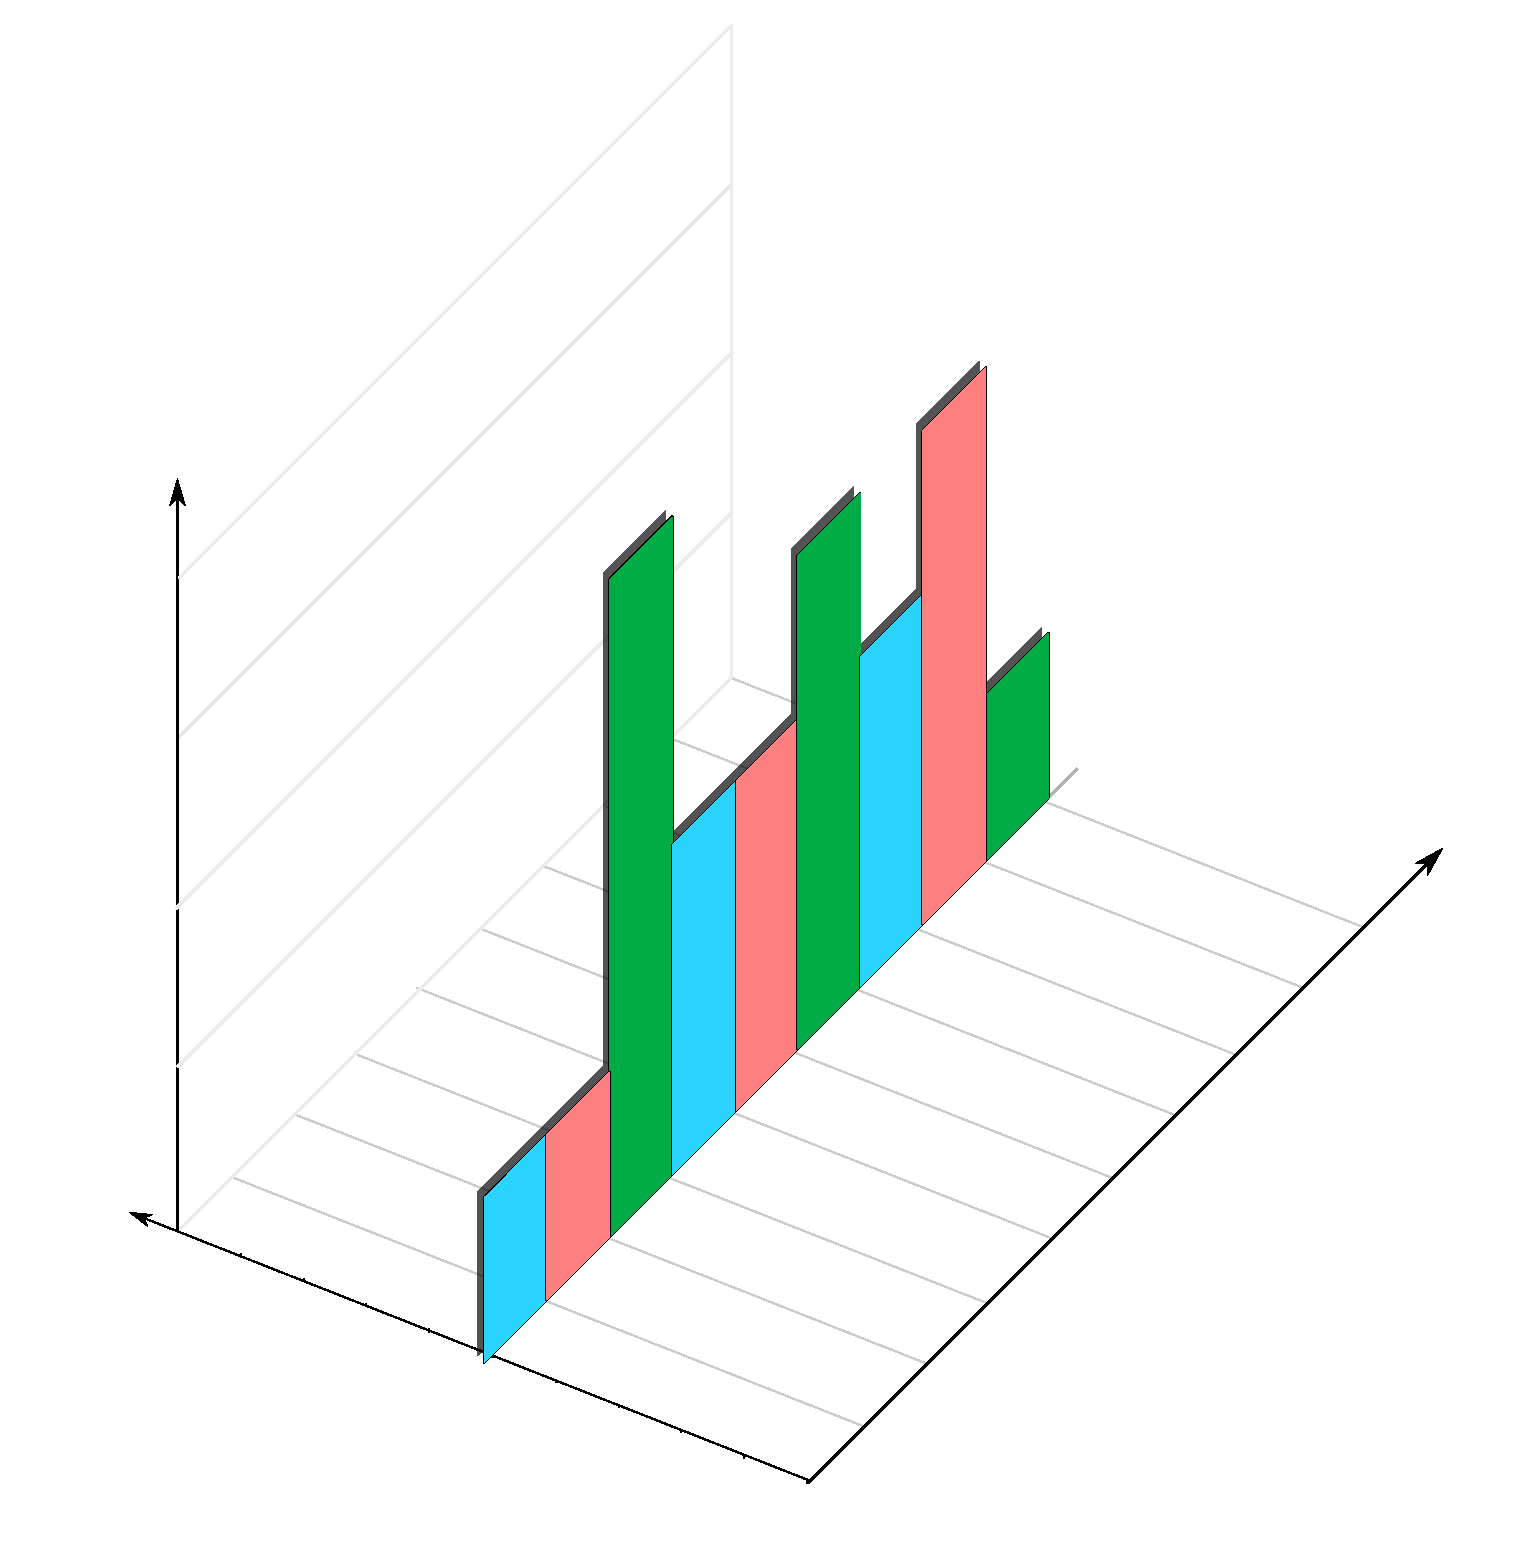
\includegraphics[width=0.95\linewidth]{serial-carrier.pdf}
        \caption{Single carrier with a higher data-rate}
        \label{fig:serial-carrier}
    \end{subfigure}%
    ~ 
    \begin{subfigure}[t]{0.48\textwidth}
        \centering
        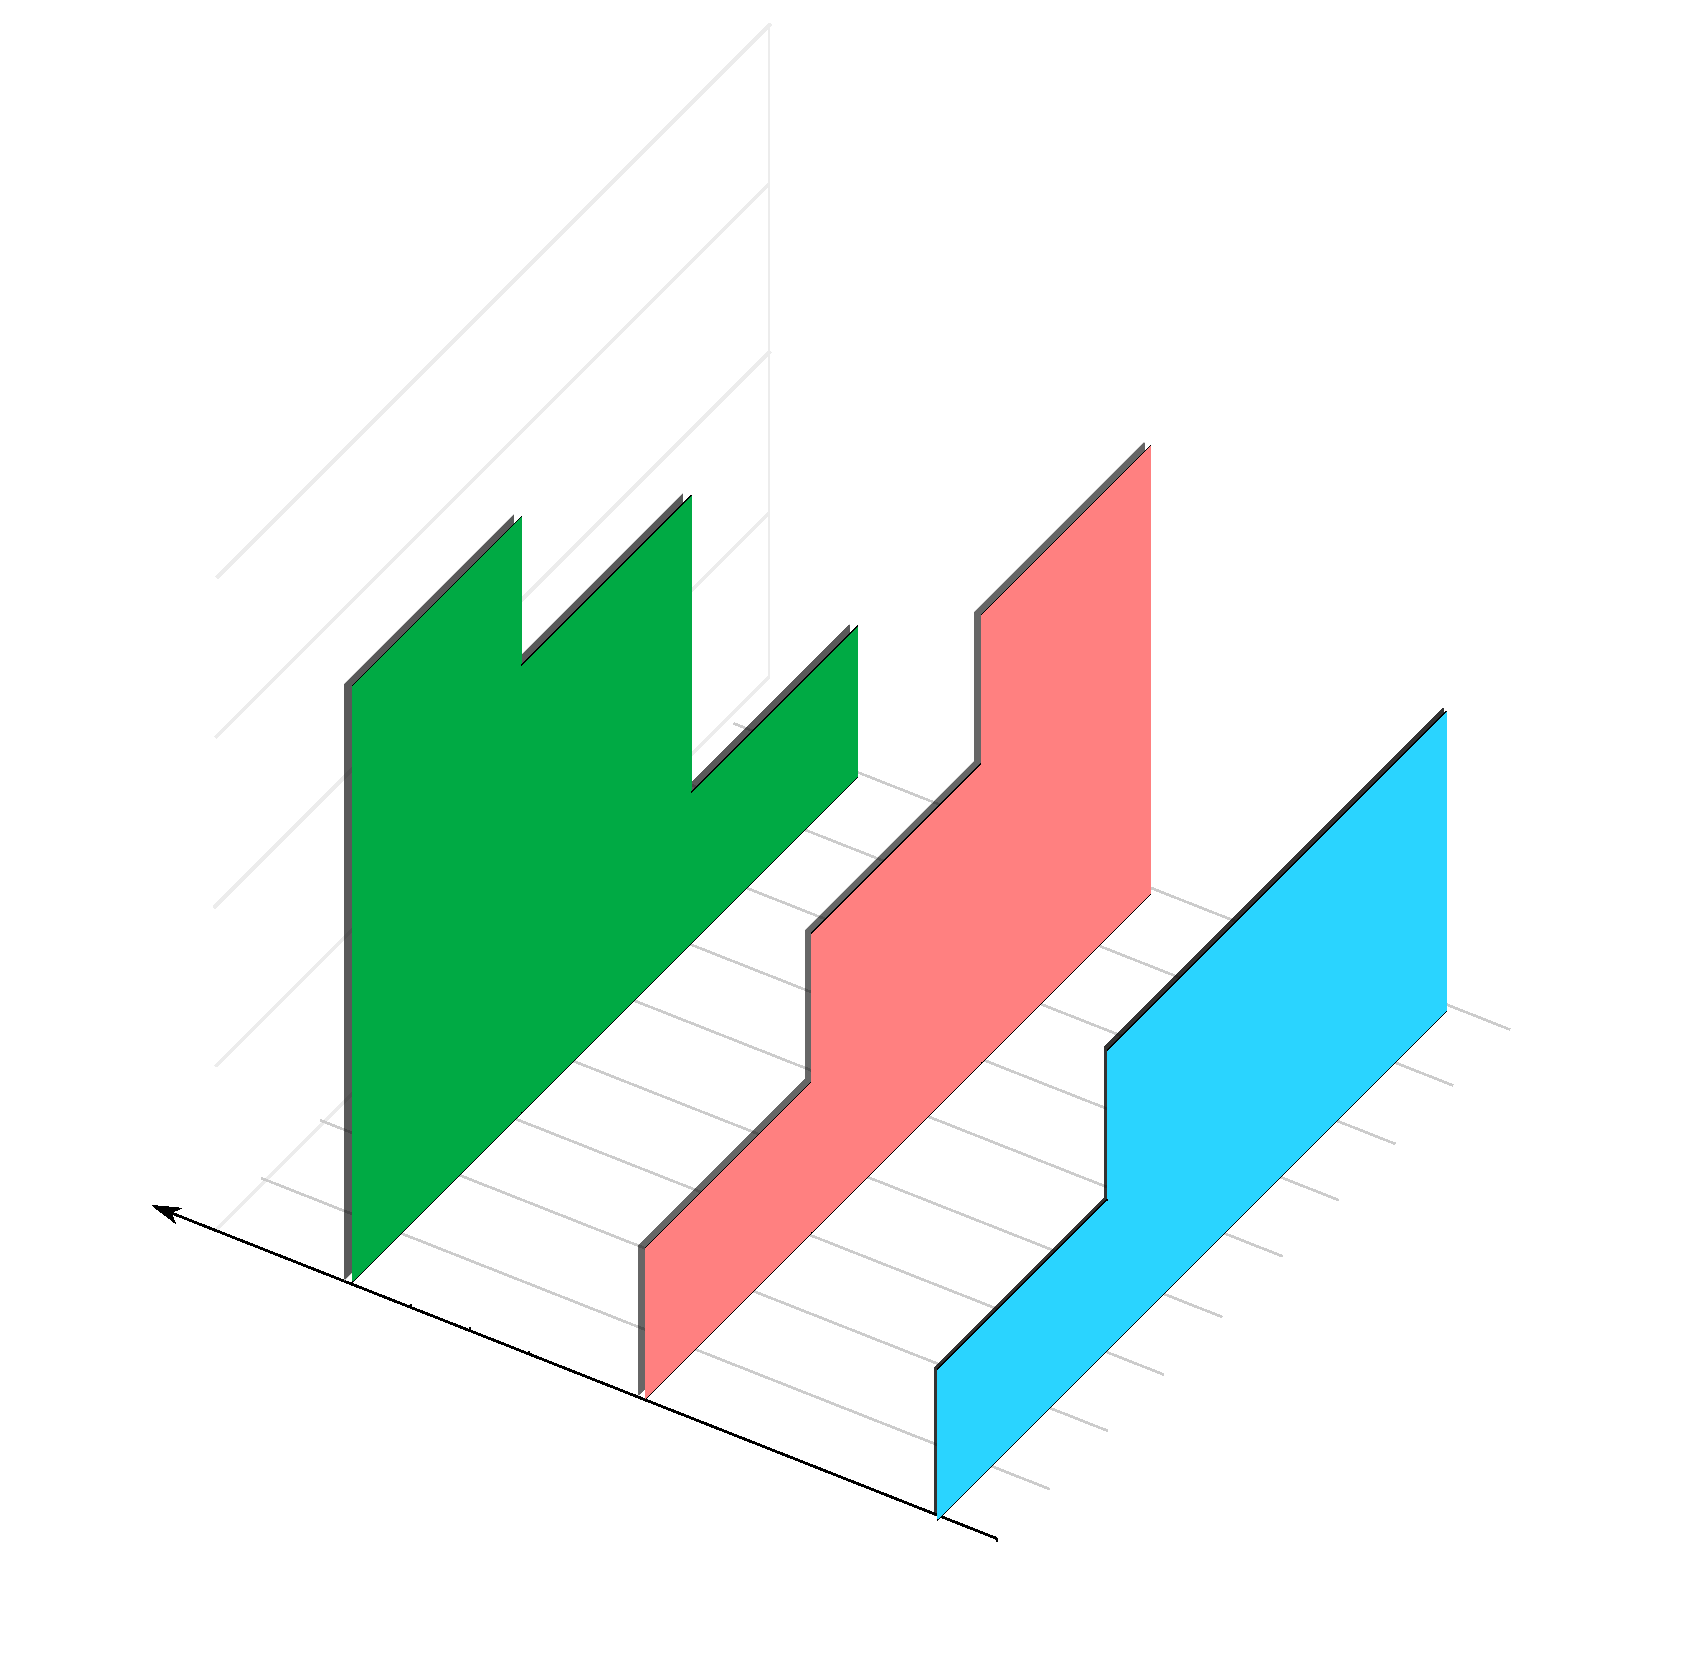
\includegraphics[width=0.9\linewidth]{parallel-carrier.pdf}
        \caption{Multiple carriers with a lower data-rate}
        \label{fig:parallel-carrier}
    \end{subfigure}
    \caption{}
    \label{fig:carrier-illustration}
\end{figure}

Figure~\ref{fig:serial-carrier} shows the serial case, where all 9 symbols are successively modulated on the carrier wave with a frequency of \(f_0\). Figure~\ref{fig:parallel-carrier}, on the other hand, shows the parallel case, with the 9 symbols split into 3 separate groups, modulating carriers with frequencies of \((f_0 - \Delta f)\), \(f_0\), and \((f_0 + \Delta f)\) respectively. Notice the symbol period for the latter situation is 3 times longer than that of the former.

While the serial scheme is simpler, the parallel scheme has two important advantages.

Multipath, inter-symbol interference

Frequency selective fading

\subsection{Frequency Division Multiplexing}
The illustration from figure~\ref{fig:carrier-illustration} was an example of \gls{fdm}, where the frequency domain is divided into separate regions, each carrying independent information. There is one caveat with this example, however. The frequency components, as shown, were assumed to be impulsive; whereas, in fact, this cannot be the case. If each component was indeed an impulse, adjacent carriers would be infinitely close to each other without interference. Instead, each carrier has an associated spectrum, and this spectrum influences the ability for one to demodulate the other carriers.

Suppose one has three carriers, each with a \(\textrm{Sa}(\omega) = \frac{\sin \omega}{\omega}\) spectrum. If the centre frequencies of these carriers are sufficiently distant from the others, there will be negligible interference from one spectrum's sidelobes to another spectrum's mainlobe. This is seen in figure~\ref{fig:three-sincs-good-distance}.


\begin{figure}
    \centering
    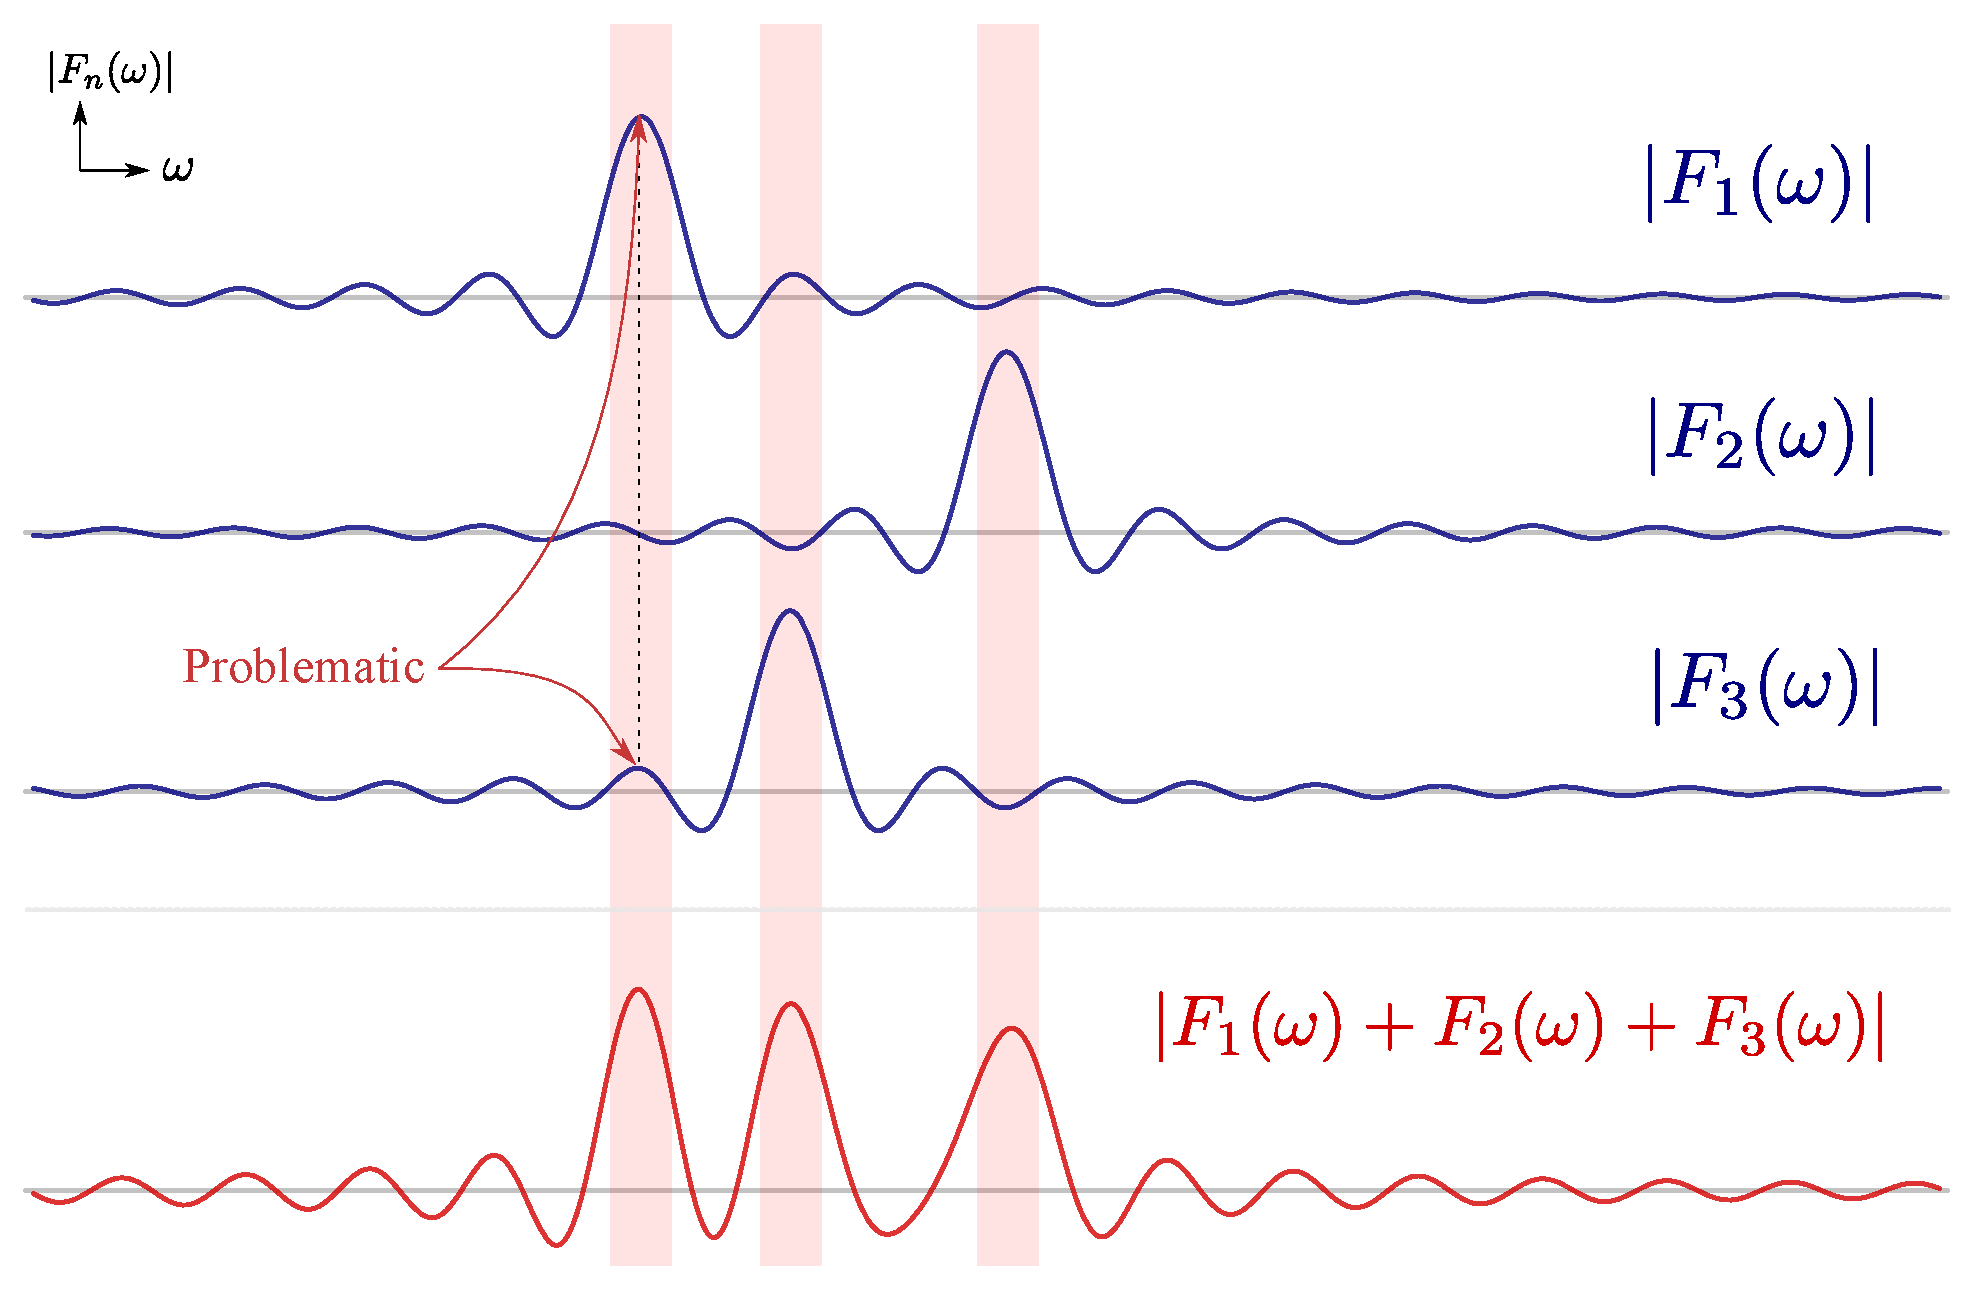
\includegraphics[width=\linewidth]{three-sincs-bad-distance.pdf}
    \caption{Three spectra spaced insufficiently far away from each other}
    \label{fig:three-sincs-bad-distance}
\end{figure}

\begin{figure}
    \centering
    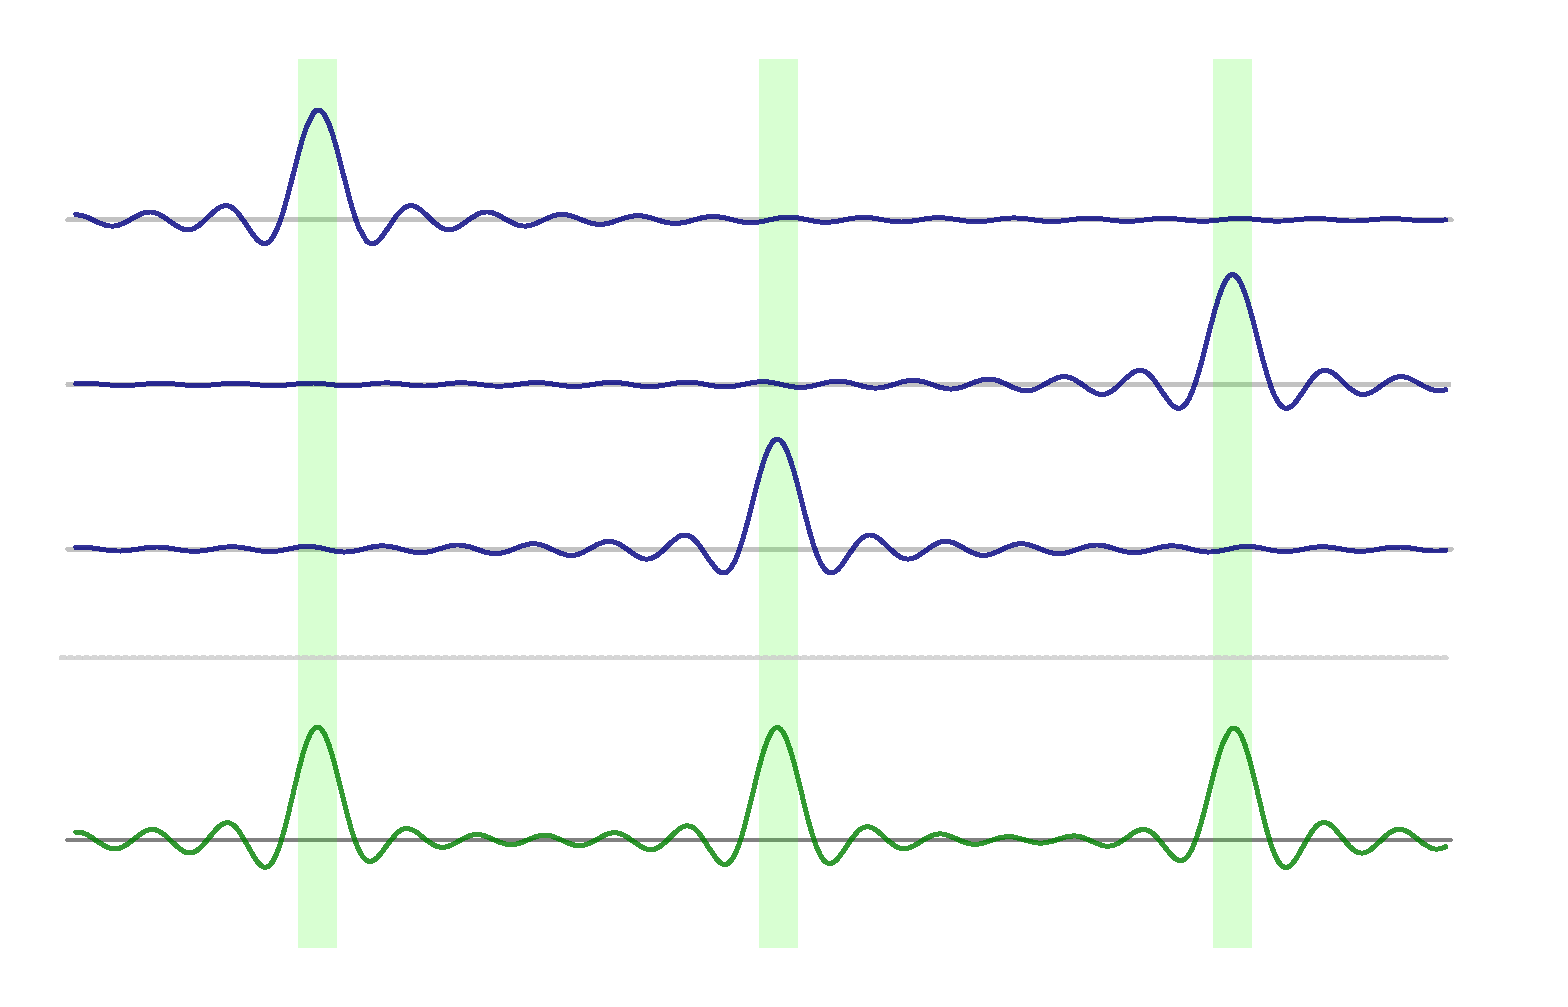
\includegraphics[width=\linewidth]{three-sincs-good-distance.pdf}
    \caption{Three spectra spaced sufficiently far away from each other}
    \label{fig:three-sincs-good-distance}
\end{figure}



\subsection{Orthogonal Carriers}


\begin{figure}
    \centering
    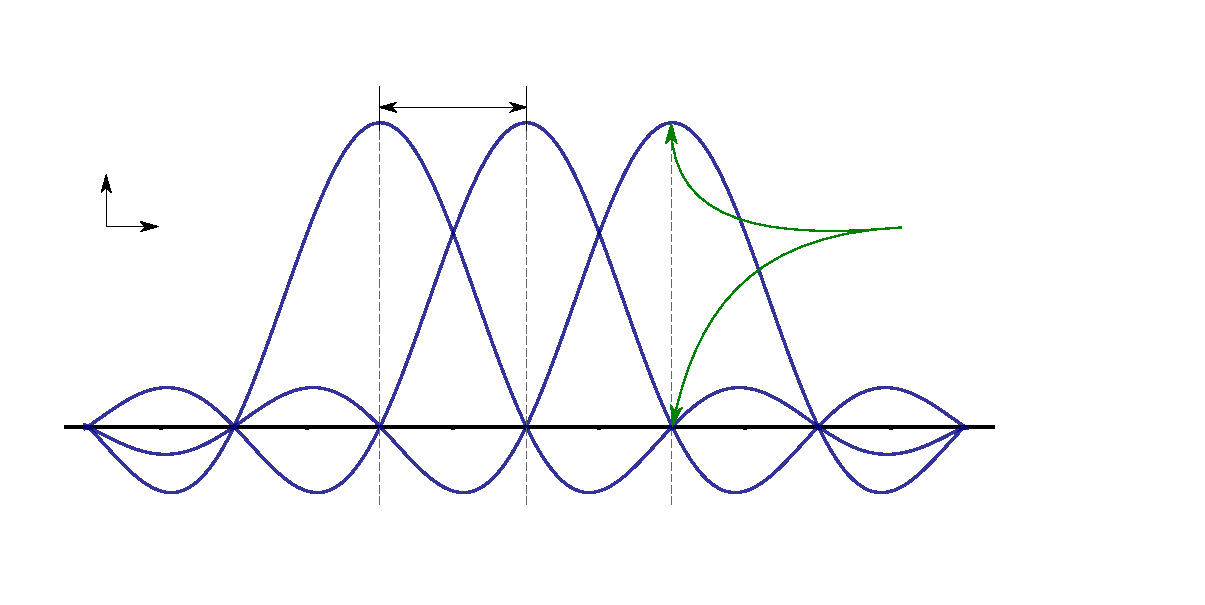
\includegraphics[width=\linewidth]{ofdm-three-sincs.pdf}
    \caption{Three spectra arranged orthogonally}
    \label{fig:ofdm-three-sincs}
\end{figure}


\subsection{Time \& Frequency Interleaving}


\subsection{Forward Error Correction}



\section{Phase Shift Keying}
\subsection{Motivation}
\subsection{Quadrature Phase Shift Keying}
\subsection{Differential Quadrature Phase Shift Keying}


\section{Transmission Frame}


\subsection{Overview}


\subsection{Null Symbol}


\subsection{Phase Reference Symbol}


\subsection{Data-carrying Symbols}


\subsection{Guard Intervals}



\section{Summary}


% ----------------------------------------------------
\ifstandalone
\bibliography{../Bibliography/References.bib}
\printnoidxglossary[type=\acronymtype,nonumberlist]
\fi
\end{document}
% ----------------------------------------------------